
Unless otherwise stated, Chapter 4 reports the supplied pre-/post-DBS image-level label task. Image-level metrics, ROI comparisons, calibration, and robustness checks are interpreted within that supplied-label setting.


\section{Dataset and Data Quality}
\begin{figure}[htbp]
\centering
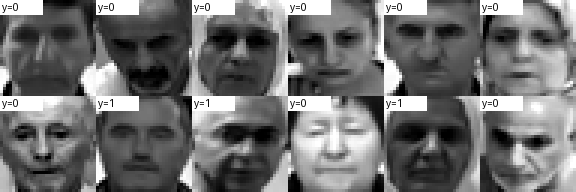
\includegraphics[width=0.72\textwidth]{figures/pd_dbs_smoke_samples.png}
\caption{PD-DBS data-loading smoke-test samples reconstructed from the local MATLAB file. The figure supports the data QC step and confirms that the 32$\times$32 grayscale inputs are visually interpretable as face images.}
\end{figure}
\begin{figure}[htbp]
\centering
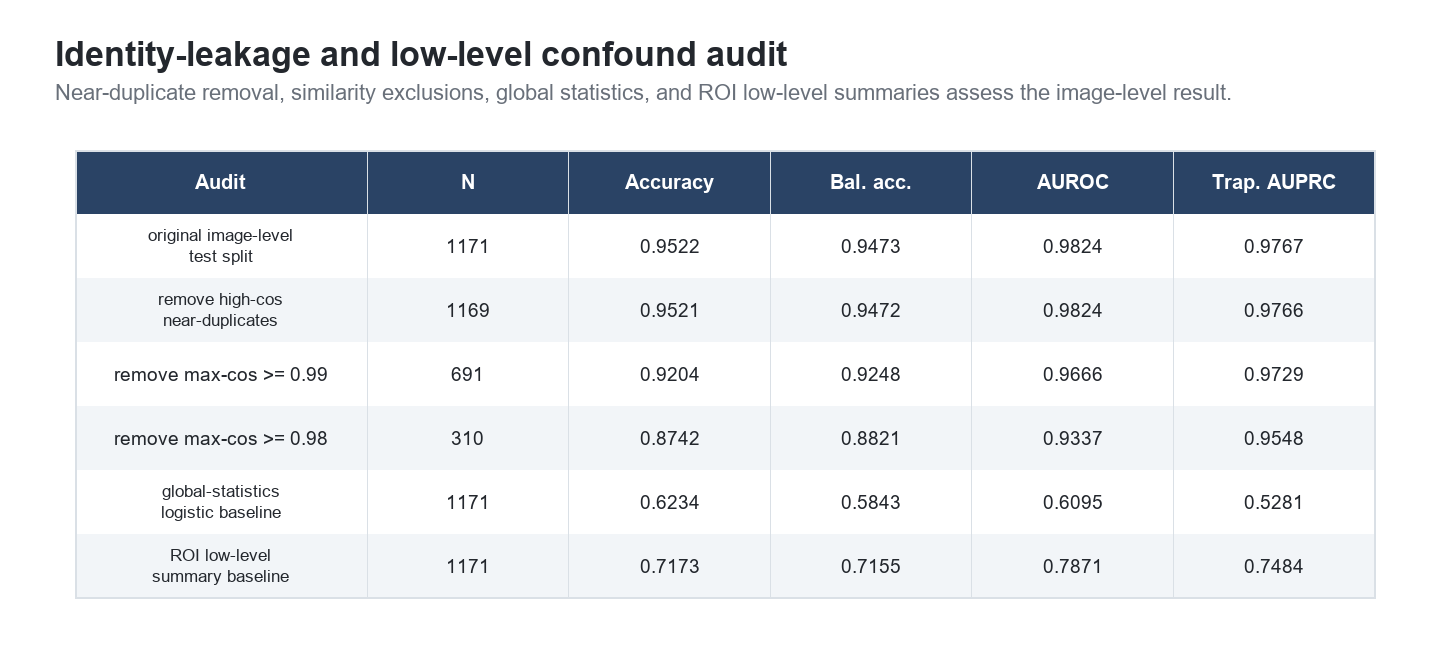
\includegraphics[width=0.95\textwidth]{figures/dissertation/fig_identity_leakage_audit.png}
\caption{Identity-leakage and low-level confound audit. The panel combines high-cosine near-duplicate removal, broader cosine-similarity exclusions, a global-statistics baseline, and an ROI low-level baseline for the supplied image-level test setting.}
\end{figure}

The dataset size, split, image resolution, and label convention are defined in Chapter 3. This section reports the corresponding QC and modelling results.


Duplicate QC found no exact train-test duplicate pairs and no near-duplicate pairs under MSE $\leq 10^{-5}$. Two high-cosine near-duplicate pairs were detected using cosine $\geq 0.999$. Removing these flagged samples left baseline metrics essentially unchanged.


The QC results confirm that the 32$\times$32 arrays are visually interpretable as facial images and can support a coarse ROI audit. The label-task evidence is evaluated through the classifier and audit analyses below.


Exact-duplicate QC found zero train-test duplicate pairs, addressing the simplest train-test leakage check. Subject-level leakage remains possible. Multiple images from the same person can differ enough to avoid exact or near-identical matching and still allow identity-like recognition. Broader similarity-based leakage and confound sensitivity were assessed beyond duplicate removal.


Progressively excluding test samples with high maximum cosine similarity to the training set reduced performance as the exclusion became stricter. Removing the two high-cosine cases left headline metrics essentially unchanged. Removing samples with max-cosine $\geq$ 0.99 left 691 test images and gave AUROC 0.9666. The max-cosine $\geq$ 0.98 rule left 310 test images and gave AUROC 0.9337. Broader similarity-threshold analyses therefore show some split sensitivity.


A global-statistics logistic baseline using eight brightness, contrast, and framing summaries achieved 0.6234 accuracy, 0.5843 balanced accuracy, and 0.6095 AUROC. The strongest single global-statistic/label correlation was upper-minus-lower mean intensity on the test split, r = -0.1429. A per-ROI low-level baseline using 40 intensity and texture summaries achieved 0.7173 accuracy, 0.7155 balanced accuracy, and 0.7871 AUROC. These results show substantial label-associated signal in low-level regional summaries.


Coarse alignment QC supported the fixed-ROI assumption at a broad level. Estimated intensity centroids were similar across train and test splits, with mean x-centroid 16.15 in train and 16.17 in test, and mean y-centroid 13.78 in train and 13.78 in test. Bounding boxes usually spanned most of the 32$\times$32 grid. This supports approximate centring and framing. The ROI analysis is therefore reported as coarse region evidence.


The 32$\times$32 resolution motivates both the validation scope and the coarse-ROI AEV design. The images are visually interpretable. The analysis therefore uses broad regions matched to the pixel grid.


\section{Baseline Pre-/Post-DBS Classification}

\begin{table}[htbp]
\centering
\scriptsize
\caption{Baseline NumPy MLP performance on the supplied image-level split. Under progressive similarity exclusion the headline AUROC of 0.9824 falls to 0.9666 (max-cosine $\geq$ 0.99, n = 691) and 0.9337 (max-cosine $\geq$ 0.98, n = 310). See Section 4.1.}
\begin{tabularx}{\textwidth}{>{\raggedright\arraybackslash}X>{\raggedright\arraybackslash}X}
\toprule
Metric & Value \\
\midrule
Majority baseline accuracy & 0.5764 \\
Accuracy & 0.9522 \\
Balanced accuracy & 0.9473 \\
F1 class 1 & 0.9419 \\
AUROC & 0.9824 \\
Trapezoidal AUPRC & 0.9767 \\
Brier score & 0.0402 \\
\bottomrule
\end{tabularx}
\end{table}

\begin{table}[htbp]
\centering
\scriptsize
\caption{Test-set confusion matrix}
\begin{tabularx}{\textwidth}{>{\raggedright\arraybackslash}X>{\raggedright\arraybackslash}X>{\raggedright\arraybackslash}X}
\toprule
 & Pred 0 & Pred 1 \\
\midrule
True 0 & 661 & 14 \\
True 1 & 42 & 454 \\
\bottomrule
\end{tabularx}
\end{table}
\begin{figure}[t]
\centering
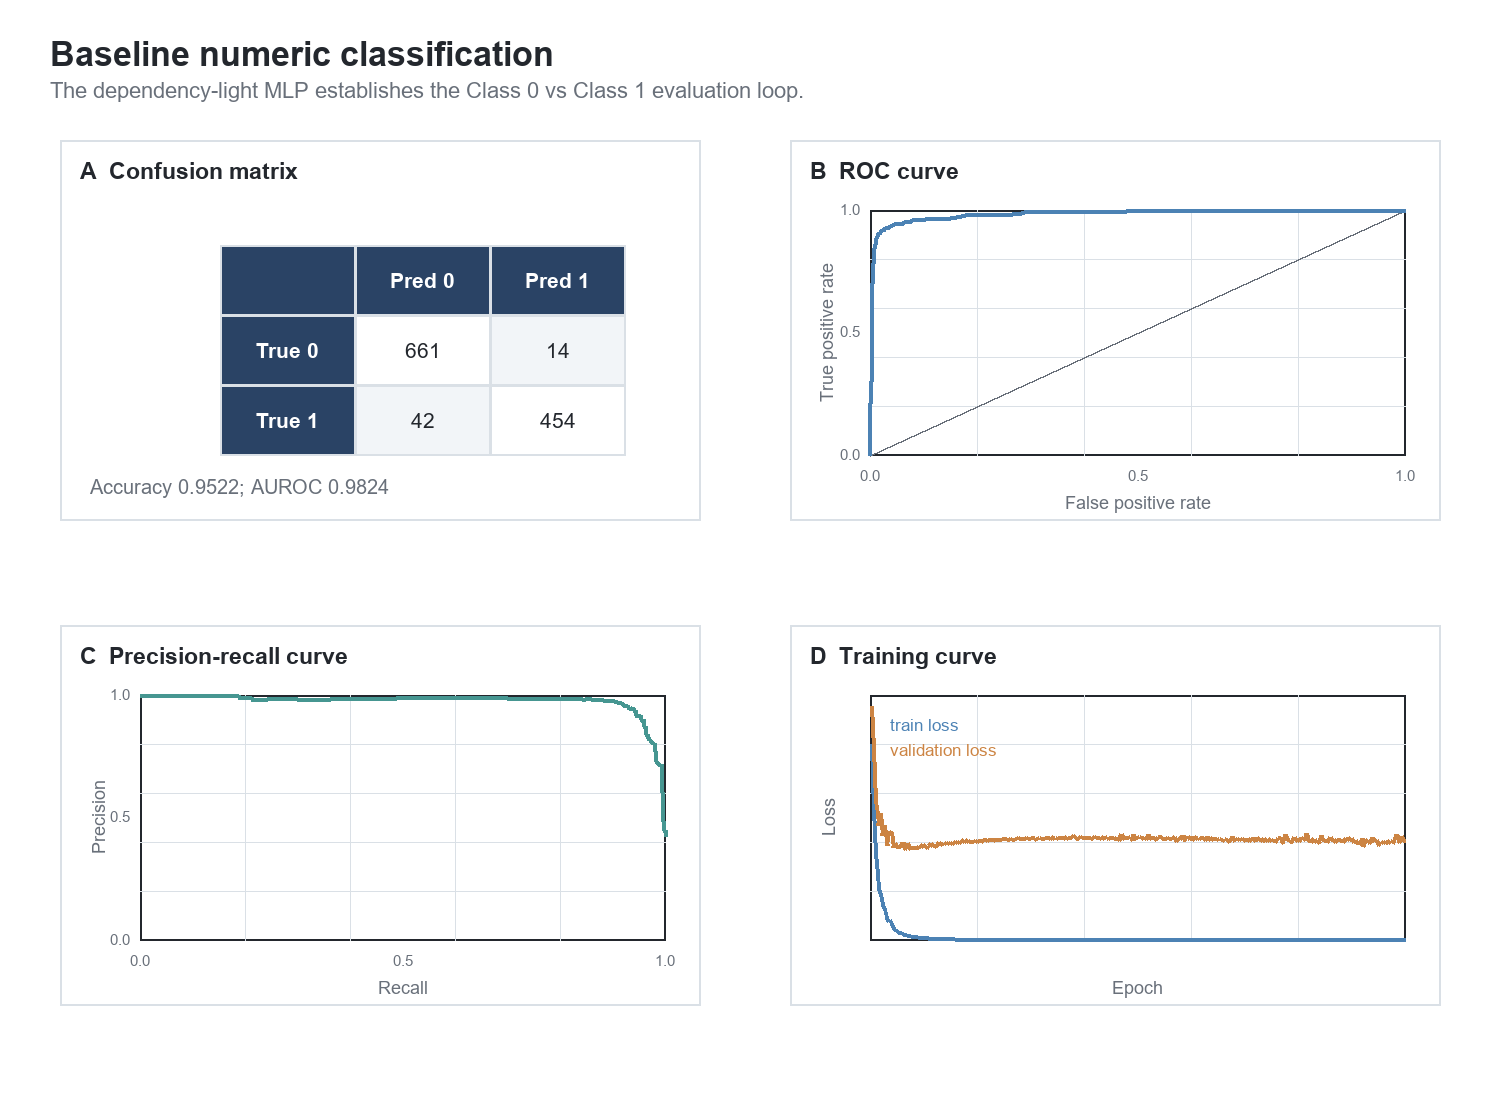
\includegraphics[width=1.00\textwidth]{figures/dissertation/fig_baseline_panel.png}
\caption{Baseline pre-/post-DBS evaluation. The panel summarises the confusion matrix, ROC curve, precision-recall curve and training curve for the dependency-light NumPy MLP baseline.}
\end{figure}

These results establish a strong supplied-split image-level baseline. A compact CNN secondary image model reached 0.9744 accuracy, 0.9727 balanced accuracy, and 0.9951 AUROC on the same supplied split. The CNN also captured the supplied split signal. The locked MLP provides the saved probabilities used for AEV, calibration, low-level, and region-only outputs. The 0.9824 AUROC is reported for the supplied image-level split.


The model substantially exceeded the majority-class baseline. The high balanced accuracy indicates strong performance on both numeric classes.


AUROC and AUPRC show strong ranking and precision-recall behaviour. At the selected threshold, the confusion matrix shows more missed Class 1 samples than incorrect Class 1 assignments for Class 0 samples. This threshold-specific behaviour describes the classifier on the supplied image-level split.


\section{Calibration}
The Brier score was 0.0402 and ECE with 10 equal-width bins was 0.0231. The mean predicted Class 1 probability was 0.4056, and the observed Class 1 fraction was 0.4236. These values indicate no gross miscalibration on the supplied pre-/post-DBS label task.


The reliability curve shows that the model's predicted probabilities broadly track observed Class 1 frequencies across bins. Because AEV is based on confidence change after perturbation, this calibration result supports the numerical use of confidence-drop scores.


In the following AEV analyses, confidence-drop scores use these same unscaled probabilities and supplied labels.

\begin{figure}[t]
\centering
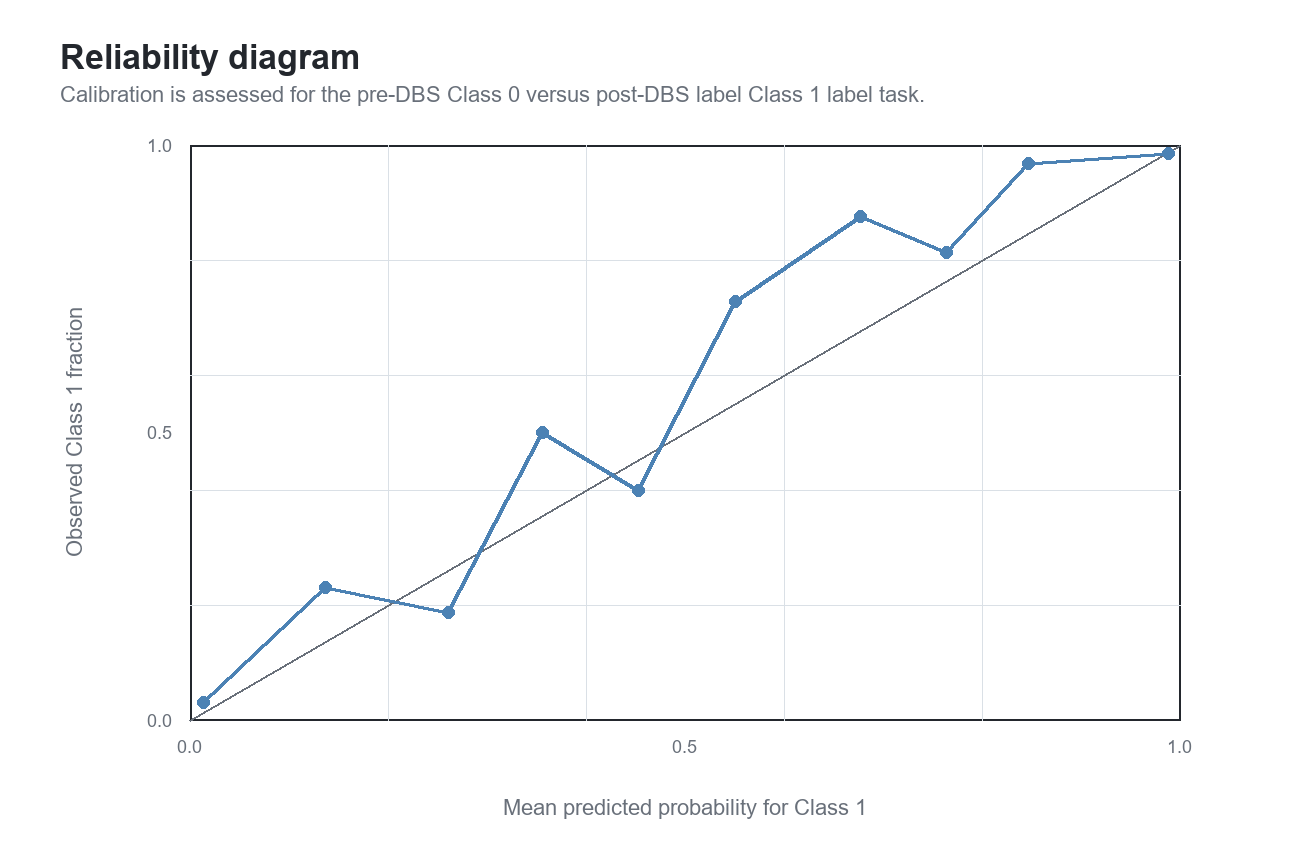
\includegraphics[width=0.66\textwidth]{figures/dissertation/fig_calibration_reliability.png}
\caption{Reliability diagram for the supplied pre-/post-DBS label task.}
\end{figure}


\section{Coarse ROI Design}
The implemented atlas used eight coarse fixed ROIs on the 32$\times$32 grayscale image grid. This scale matched the low-resolution setting.


The final ROI masks were mutually exclusive, with zero overlapping pixels. This avoided duplicated evidence around the cheek and mouth boundaries.


The eight ROIs cover 840 pixels of the 1024-pixel image grid. Unassigned pixels mainly include border and background areas, so the masks focus on interpretable facial regions.


The coarse ROI design is a fixed-region atlas for the available 32$\times$32 images. It demonstrates the AEV workflow in a low-resolution setting. A higher-resolution future dataset could support a more detailed craniofacial atlas with separate brow, orbital, nasal, philtrum, lip, chin, mandibular, and cheek regions.

\begin{figure}[H]
\centering
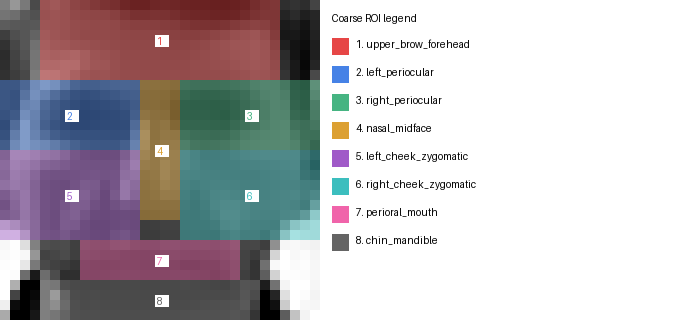
\includegraphics[width=0.62\textwidth]{outputs/roi/coarse_roi_overlay_examples.png}
\caption{Mutually exclusive coarse ROI overlay for the 32$\times$32 image grid. The low-resolution ROI design uses broad facial regions matched to the available image detail.}
\end{figure}


\section{Occlusion-Based AEV}
\begin{figure}[htbp]
\centering
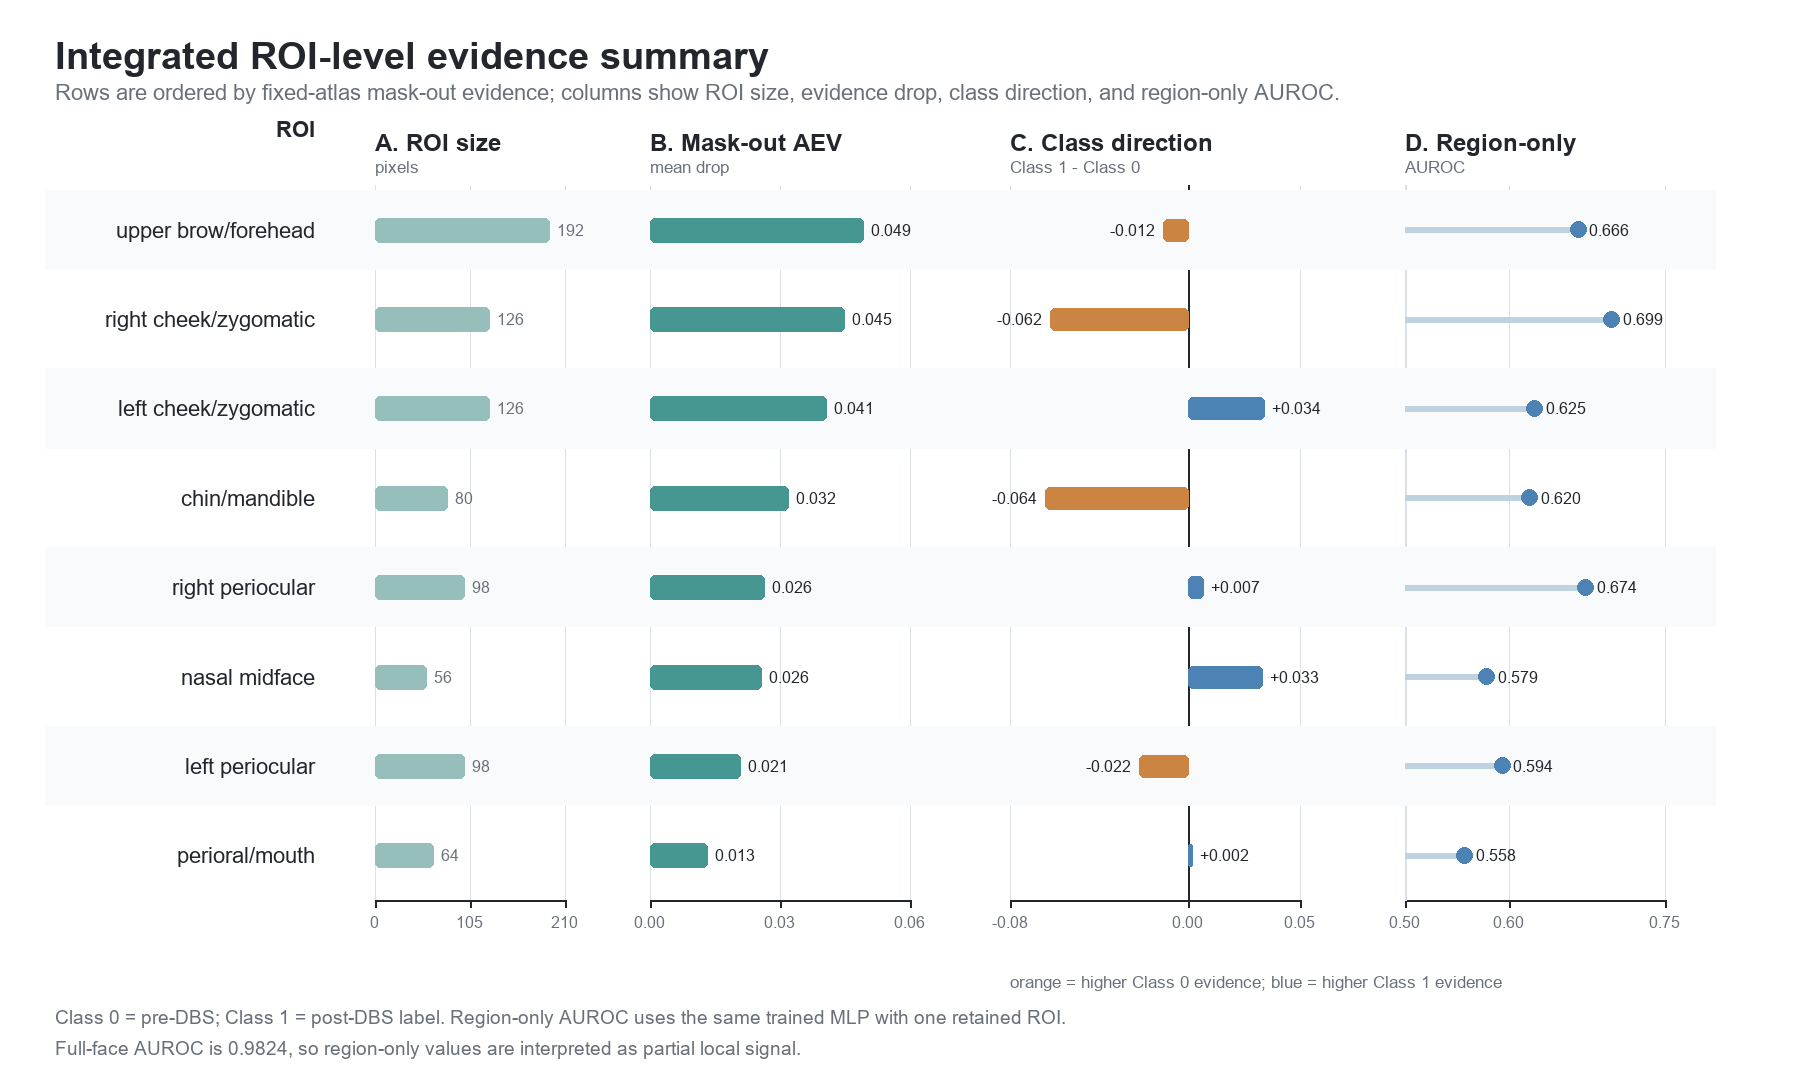
\includegraphics[width=0.98\textwidth]{figures/dissertation/fig_roi_evidence_summary.png}
\caption{Integrated ROI-level evidence summary. Rows are ordered by fixed-atlas mask-out AEV. Columns show ROI size, mean true-class confidence drop, Class 1 minus Class 0 evidence difference, and same-MLP region-only AUROC.}
\end{figure}

\begin{table}[htbp]
\centering
\scriptsize
\caption{Largest raw mean true-class confidence drops under fixed-atlas ROI mask-out}
\begin{tabularx}{\textwidth}{>{\raggedright\arraybackslash}X>{\raggedright\arraybackslash}X}
\toprule
ROI & Mean evidence drop \\
\midrule
\texttt{\detokenize{upper_brow_forehead}} & 0.049135 \\
\texttt{\detokenize{right_cheek_zygomatic}} & 0.044752 \\
\texttt{\detokenize{left_cheek_zygomatic}} & 0.040594 \\
\texttt{\detokenize{chin_mandible}} & 0.031842 \\
\bottomrule
\end{tabularx}
\end{table}

These ROIs produced the largest raw reductions in true-class confidence under mask-out testing, indicating that masking them had the strongest complete-region effect on the model's confidence in the true numeric class.


Raw full-region AEV scores were strongly associated with ROI size. Across the eight fixed ROIs, Pearson correlation between ROI pixel count and raw mean drop was 0.8307, and Spearman rank correlation was 0.8073. This means that the raw ranking is best read as total perturbation effect for a complete named region.


\begin{table}[htbp]
\centering
\scriptsize
\caption{Fixed-atlas AEV size-normalized sensitivity summary}
\begin{tabularx}{\textwidth}{>{\raggedright\arraybackslash}X>{\raggedright\arraybackslash}X>{\raggedright\arraybackslash}X>{\raggedright\arraybackslash}X>{\raggedright\arraybackslash}X}
\toprule
ROI & Pixels & Raw mean drop & Raw rank & Drop per 100 pixels / rank \\
\midrule
Nasal midface & 56 & 0.025674 & 6 & 0.045846 / 1 \\
Chin/mandible & 80 & 0.031842 & 4 & 0.039802 / 2 \\
Right cheek/zygomatic & 126 & 0.044752 & 2 & 0.035518 / 3 \\
Left cheek/zygomatic & 126 & 0.040594 & 3 & 0.032218 / 4 \\
Right periocular & 98 & 0.026388 & 5 & 0.026927 / 5 \\
Upper brow/forehead & 192 & 0.049135 & 1 & 0.025591 / 6 \\
Left periocular & 98 & 0.020829 & 7 & 0.021254 / 7 \\
Perioral/mouth & 64 & 0.013141 & 8 & 0.020534 / 8 \\
\bottomrule
\end{tabularx}
\end{table}


The size-normalized sensitivity check changed the ranking. Nasal midface and chin/mandible moved upward after dividing by pixel count. Upper brow/forehead moved from the highest raw mean drop to sixth by drop per 100 pixels. The perioral/mouth region stayed lowest in both summaries.


Evidence-drop values are true-class confidence changes after region masking. A high evidence drop means that replacing a region with training-set mean values reduced the classifier's confidence in the true numeric label.


The raw and normalized summaries therefore answer different measurement questions. Raw AEV reports the total effect of masking a full ROI. The size-normalized ranking is the primary lens for comparing evidence intensity across ROIs of different sizes, because raw drops scale with ROI pixel count. Region-only validation, YuNet sensitivity, and perturbation tests provide additional context for these fixed-ROI measurements.


\section{Class-Specific AEV Statistics}

\begin{table}[htbp]
\centering
\scriptsize
\caption{Fixed-atlas AEV class-specific statistics on the supplied split}
\begin{tabularx}{\textwidth}{>{\raggedright\arraybackslash}X>{\raggedright\arraybackslash}X>{\raggedright\arraybackslash}X>{\raggedright\arraybackslash}X>{\raggedright\arraybackslash}X>{\raggedright\arraybackslash}X}
\toprule
ROI & Direction & Difference [95\% CI] & Cohen d & Cliff delta & FDR \\
\midrule
Chin/mandible & higher in Class 0 & -0.0645 [-0.0795, -0.0496] & -0.4792 & -0.3397 & 0.0005 \\
Right cheek/zygomatic & higher in Class 0 & -0.0622 [-0.0805, -0.0440] & -0.3786 & -0.2943 & 0.0005 \\
Left cheek/zygomatic & higher in Class 1 & 0.0340 [0.0125, 0.0556] & 0.1953 & 0.0111 & 0.0022 \\
Nasal midface & higher in Class 1 & 0.0328 [0.0189, 0.0480] & 0.2769 & 0.1885 & 0.0005 \\
Left periocular & higher in Class 0 & -0.0223 [-0.0352, -0.0098] & -0.2048 & -0.2049 & 0.0022 \\
Upper brow/forehead & higher in Class 0 & -0.0116 [-0.0307, 0.0081] & -0.0711 & 0.0047 & 0.3026 \\
Right periocular & higher in Class 1 & 0.0067 [-0.0068, 0.0202] & 0.0587 & 0.1259 & 0.3709 \\
Perioral/mouth & higher in Class 1 & 0.0017 [-0.0100, 0.0131] & 0.0189 & -0.1252 & 0.7544 \\
\bottomrule
\end{tabularx}
\end{table}

Class-specific analysis adds directionality to the global importance ranking. Chin/mandible, right cheek/zygomatic, and left periocular evidence were higher in Class 0. Left cheek/zygomatic and nasal midface evidence were higher in Class 1. The difference is defined as Class 1 minus Class 0. Negative values indicate higher pre-DBS evidence, and positive values indicate higher supplied post-DBS label evidence. Five ROIs remained significant after FDR correction. The remaining three ROIs are reported as non-significant supplied-split estimates.


Together, the supplied-split class statistics show how AEV turns explanation into an auditable statistical object. Regional evidence can be ranked, tested, assigned effect sizes, and checked with confidence intervals. The reported AEV directions are supplied-split findings and are read alongside the low-level confound baselines.


\section{Region-Only Validation}
The best region-only ROI was \texttt{\detokenize{right_cheek_zygomatic}}, with 0.6763 accuracy, 0.6551 balanced accuracy, and 0.6988 AUROC. Region-only validation tests the fixed MLP response when one ROI is retained. The best retained-region response was lower than the full-face AUROC of 0.9824 and the ROI low-level summary baseline AUROC of 0.7871. Simple regional intensity and texture summaries carried stronger label-ranking signal than any single retained fixed ROI.


The right cheek/zygomatic region ranked highest in region-only validation and also appeared among the strongest raw occlusion regions. This agreement identifies a stable retained-region response for the supplied label task. The gap between region-only, low-level ROI baseline, and full-face performance is an audit finding. AEV records how the trained model responds to named-region perturbations, and the low-level baseline quantifies regional intensity and texture signal.


As an automatic ROI-definition sensitivity check, YuNet was run after upsampling the 32$\times$32 images to 256$\times$256. YuNet detected all 2343 faces. The main region-only comparison tested whether the fixed-atlas right-cheek signal persisted under automatically defined ROI boxes.

\begin{figure}[t]
\centering
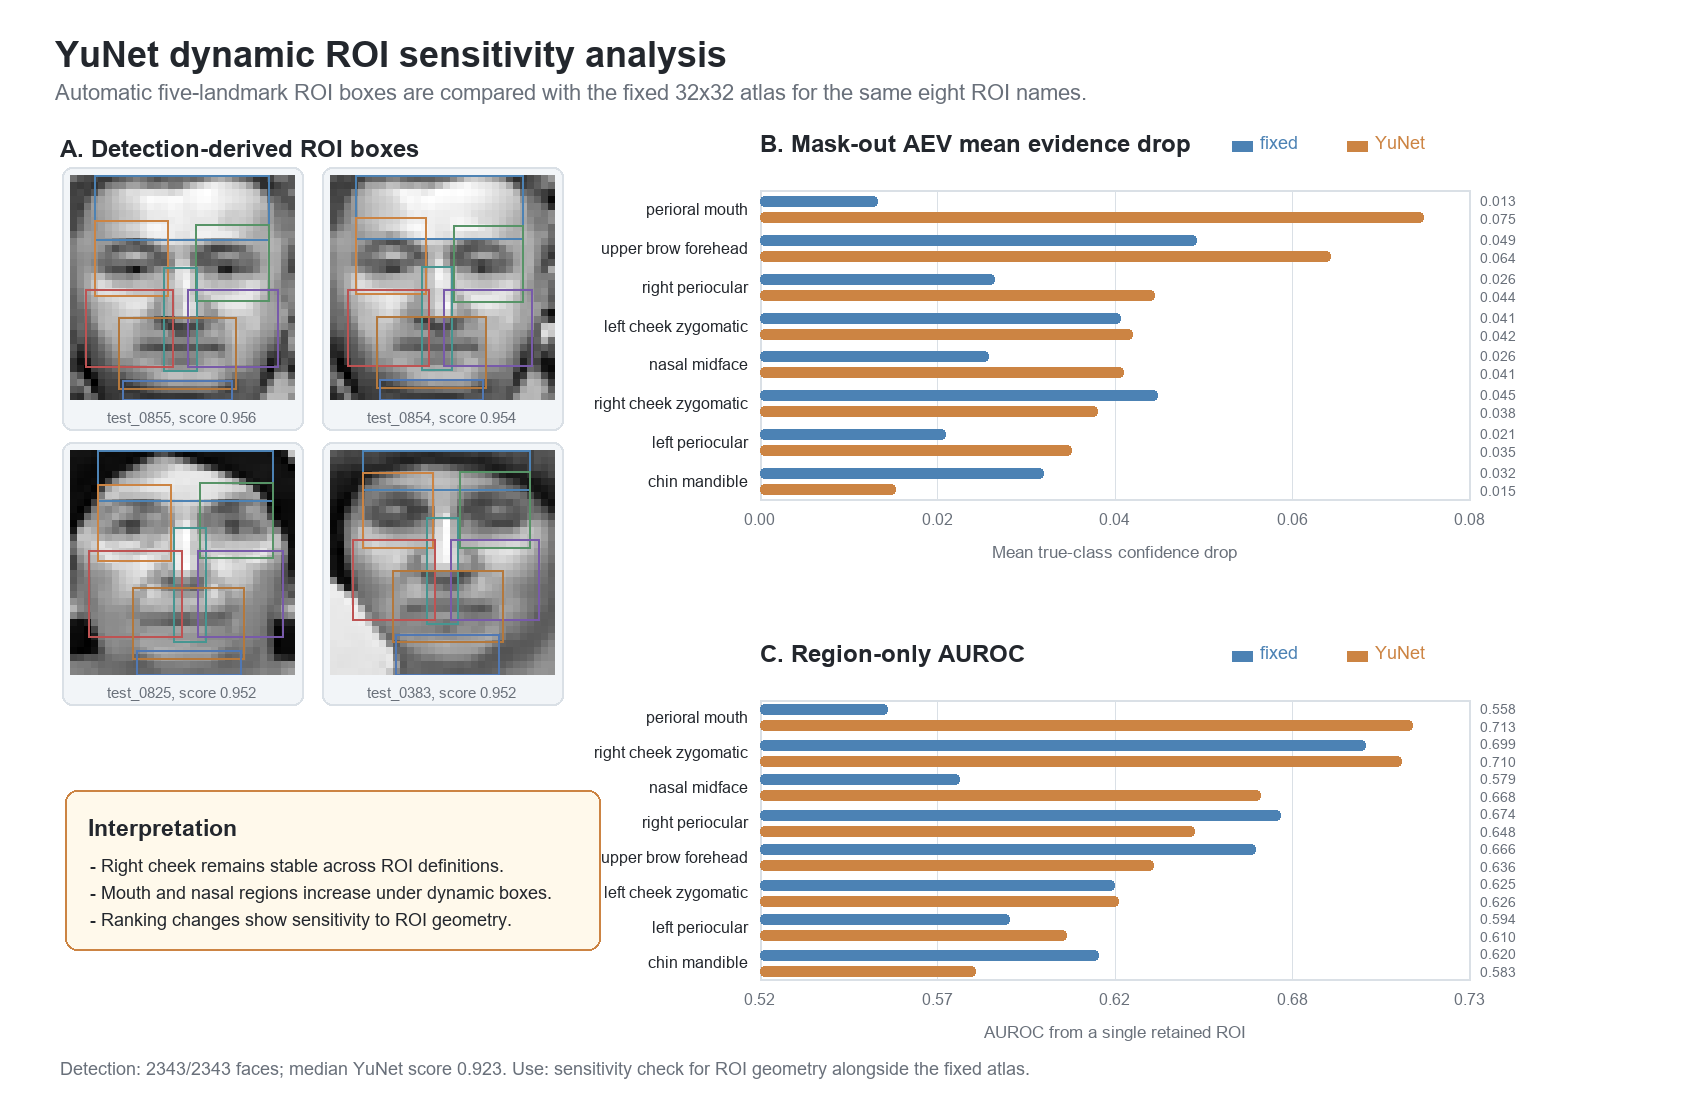
\includegraphics[width=1.00\textwidth]{figures/dissertation/fig_yunet_dynamic_roi_sensitivity.png}
\caption{YuNet dynamic ROI sensitivity analysis. Automatic five-landmark ROI boxes are compared with the fixed 32$\times$32 atlas for detection-derived ROI examples, mask-out AEV mean evidence drops, and region-only AUROC. The comparison tests ROI-geometry sensitivity.}
\end{figure}


\begin{table}[htbp]
\centering
\scriptsize
\caption{Fixed-atlas versus YuNet-derived region-only validation}
\begin{tabularx}{\textwidth}{>{\raggedright\arraybackslash}X>{\raggedright\arraybackslash}X>{\raggedright\arraybackslash}X>{\raggedright\arraybackslash}X>{\raggedright\arraybackslash}X>{\raggedright\arraybackslash}X>{\raggedright\arraybackslash}X}
\toprule
ROI & Fixed BA & Fixed AUROC & YuNet BA & YuNet AUROC & Delta BA & Delta AUROC \\
\midrule
Right cheek & 0.6551 & 0.6988 & 0.6575 & 0.7096 & 0.0024 & 0.0107 \\
Mouth & 0.5560 & 0.5577 & 0.6535 & 0.7129 & 0.0975 & 0.1552 \\
Nasal midface & 0.5548 & 0.5788 & 0.6248 & 0.6679 & 0.0700 & 0.0891 \\
\bottomrule
\end{tabularx}
\end{table}

These fixed-versus-YuNet deltas measure ROI-definition sensitivity. The model, test set, labels, fill value, and ROI names are held fixed. ROI geometry and pixel count change together when YuNet boxes replace the fixed atlas.


For right cheek/zygomatic, the YuNet-minus-fixed AUROC difference was small: delta 0.0107 with a 95\% bootstrap interval from -0.0200 to 0.0417. The balanced-accuracy delta was 0.0024 with a 95\% bootstrap interval from -0.0291 to 0.0348. A fixed-ROI jitter test gave the same top region in 10 of 11 atlas variants, and the right-cheek AUROC range across jittered variants was 0.6896 to 0.7197. These checks support the right-cheek region-only result as spatially stable under small ROI-definition changes.


YuNet dynamic AEV gave a different ranking from the fixed-atlas AEV. The largest YuNet evidence drops were perioral/mouth 0.0747, upper brow/forehead 0.0642, and right periocular 0.0444. Right cheek/zygomatic remained measurable at 0.0380. The shift is an ROI-geometry sensitivity finding. Fixed rectangular masks and detection-derived boxes capture different pixel areas, especially around the mouth. The fixed atlas is used as the primary AEV system because it gives one reproducible 32$\times$32 coordinate frame for class statistics, occlusion, region-only validation, and robustness checks.


\section{Low-Level / Full-Pixel Score Decomposition}

To examine how the full-pixel MLP score related to low-level regional image summaries, an exploratory block-wise logistic decomposition was conducted on the supplied test split. The decomposition model used five-fold out-of-fold (OOF) cross-validation within the test split. The analysis compares the incremental ranking discrimination of two fixed predictor blocks under one common audit protocol.

Under this protocol, the 40 ROI low-level summary features alone reached an out-of-fold AUROC of 0.7709, and the locked full-pixel MLP score alone reached 0.9794. Combining the two blocks gave 0.9752. Adding the full-pixel score to the low-level block increased AUROC by +0.2043. Adding the low-level block to the full-pixel score changed AUROC by -0.0042. All three values use the same out-of-fold protocol. The separately reported headline AUROC of 0.9824 (Table 4.7) is the locked model's train-to-test score. This asymmetric pattern shows that low-level ROI summaries carry measurable label-associated signal and add no ranking discrimination beyond the full-pixel MLP score in this decomposition.

The decomposition supports a two-part interpretation. First, ROI-level brightness and texture summaries contain substantial label-associated information. Second, the full-pixel MLP score captures additional split-specific structure beyond these 40 summaries. Attribution of that additional structure to facial morphology, DBS state, identity, or acquisition effects is a later patient-level analysis using identity and acquisition metadata.


\begin{table}[htbp]
\centering
\scriptsize
\caption{Low-level / full-pixel score decomposition on the supplied test split. The upper block lists the headline baselines fitted on the training split and evaluated on the test split (Section 4.1). The lower block is an exploratory five-fold out-of-fold (OOF) logistic decomposition computed within the test split. All OOF rows share one protocol and are directly comparable. The train-to-test headline AUROC is reported as a reference anchor.}
\begin{tabularx}{\textwidth}{>{\raggedright\arraybackslash}X>{\raggedright\arraybackslash}X}
\toprule
Predictor & AUROC \\
\midrule
\multicolumn{2}{l}{\textit{Headline baselines (train$\rightarrow$test fit, Section 4.1)}} \\
Majority baseline & 0.500 \\
Global image-statistics confound (8 features) & 0.6095 \\
ROI low-level confound (40 features) & 0.7871 \\
Full-pixel MLP & 0.982 \\
\midrule
\multicolumn{2}{l}{\textit{Exploratory decomposition (5-fold out-of-fold logistic, test split)}} \\
ROI low-level summaries only & 0.7709 \\
Full-pixel MLP score only & 0.9794 \\
Low-level summaries + full-pixel MLP score & 0.9752 \\
Increment of MLP score over low-level & +0.2043 \\
Increment of low-level over MLP score & -0.0042 \\
\bottomrule
\end{tabularx}
\end{table}


\section{Robustness}
\begin{figure}[htbp]
\centering
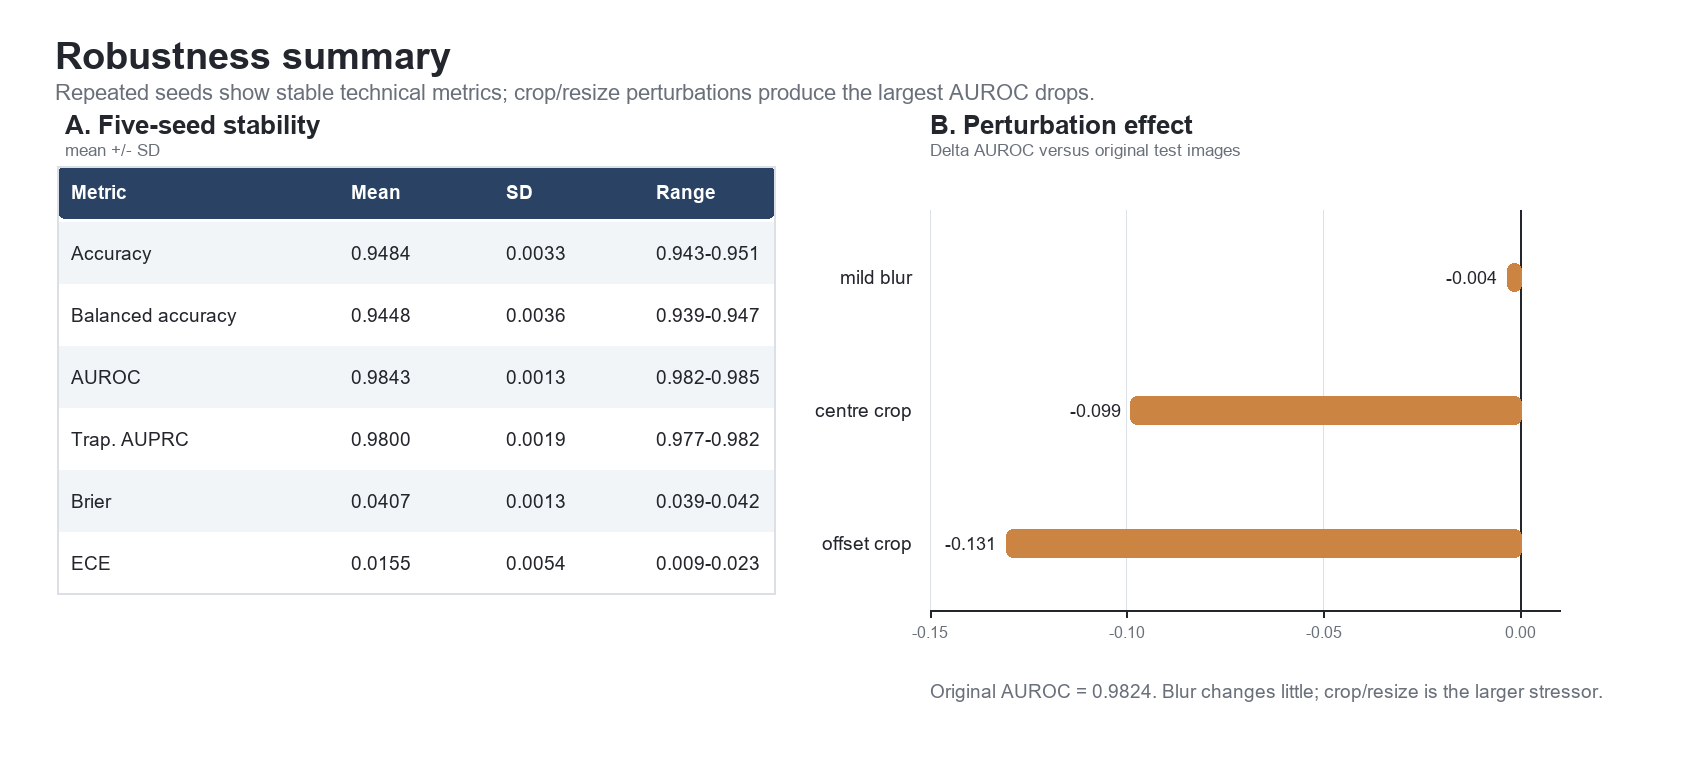
\includegraphics[width=0.98\textwidth]{figures/dissertation/fig_robustness_summary.png}
\caption{Robustness summary. Multi-seed stability is reported as mean, standard deviation, and range across repeated runs. Perturbation robustness is reported as AUROC change relative to original test images.}
\end{figure}

The headline AUROC of 0.9824 comes from the locked final run. The multi-seed values in Figure 4.8 are means across repeated validation splits and model initialisations.


The multi-seed results show stable baseline behaviour across random seeds. Accuracy, balanced accuracy, AUROC, and trapezoidal AUPRC all had small standard deviations across repeated splits and initialisations. This supports the stability of the pre-/post-DBS label classification pipeline.


The perturbation results show a more specific pattern. Mild blur had very limited effect on AUROC, with AUROC delta -0.0035 and ROI rank correlation 0.9762 with top-3 overlap of 3/3. In contrast, centre crop and offset crop reduced AUROC more substantially, with deltas of -0.0991 and -0.1307. This is expected in 32$\times$32 facial images because cropping can shift or remove a large portion of the face.


Additional ROI sensitivity checks refined the robustness picture. Label permutation reduced full-face AUROC to a near-chance mean of 0.5450 across three seeds. Occlusion fill-strategy analysis showed that zero fill produced large out-of-distribution effects. Blur fill produced very small evidence drops and unstable rankings. Training-mean fill was therefore retained for the main AEV analysis. In the MLP region-only sensitivity outputs, fixed-versus-YuNet rank correlation was weak across all eight ROIs, and the fixed and YuNet analyses agreed on right cheek/zygomatic as the top balanced-accuracy region.


\section{Compact CNN and Grad-CAM ROI Agreement}
A compact CNN was trained as a secondary image model and Grad-CAM source. On the supplied image-level split it achieved 0.9744 accuracy, 0.9727 balanced accuracy, and 0.9951 AUROC. Two independent ROI-rank comparisons gave Spearman rho = 0.9524: Grad-CAM projection versus same-CNN fixed-atlas occlusion, and same-CNN fixed-atlas occlusion versus same-CNN YuNet automatic-ROI occlusion. In both comparisons, the top-three ROI overlap was 3/3.


The 0.9524 correlations are same-CNN sanity checks: two explanation views of the compact CNN ranked the fixed ROIs similarly. Cross-model comparisons change both architecture and explanation mechanism. MLP region-mask AEV versus CNN Grad-CAM gave Spearman rho = 0.7857, and MLP region-mask AEV versus pixel-occlusion ROI aggregation gave rho = 0.3810 and 0.6429.


\begin{figure}[H]
\centering
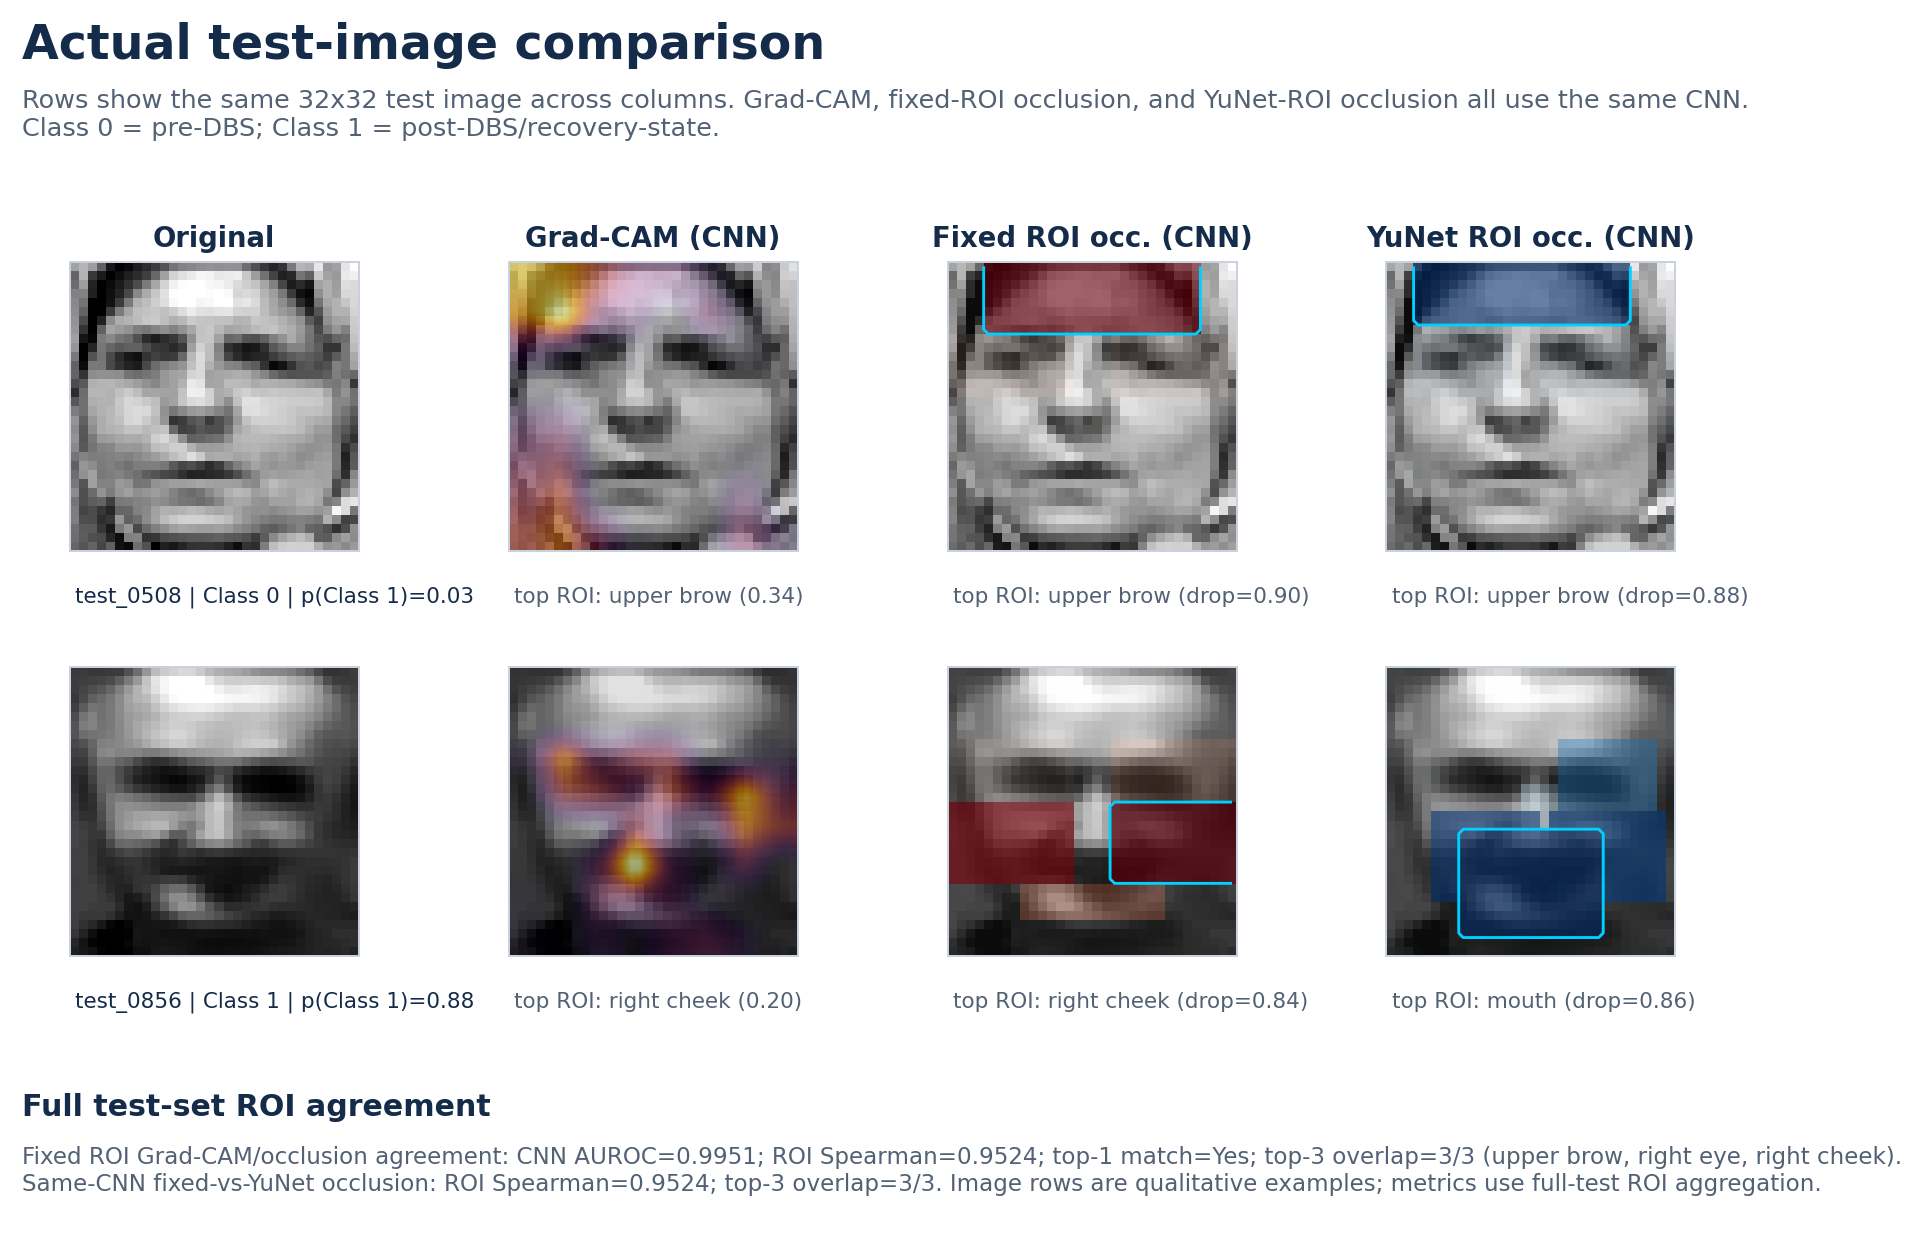
\includegraphics[width=1.00\textwidth]{figures/dissertation/fig_gradcam_occlusion_overlap.png}
\caption{Grad-CAM and ROI occlusion comparison on real test images. Each row shows the same 32$\times$32 test image as the original input, CNN Grad-CAM, CNN fixed-atlas ROI occlusion, and CNN YuNet automatic-ROI occlusion. The quantitative comparison is based on full test-set ROI aggregation.}
\end{figure}

The pixel-occlusion baseline provides a lighter perturbation comparator: each pixel was masked individually and then aggregated into the same eight ROIs. Its agreement with region-mask AEV was moderate when pixel drops were summed within ROIs. Cross-model agreement between MLP AEV and CNN Grad-CAM was moderate-to-high at ROI rank level. Same-CNN Grad-CAM versus same-CNN occlusion remained the strongest agreement.

\begin{table}[H]
\centering
\scriptsize
\caption{XAI baseline and cross-method ROI-rank comparisons}
\begin{tabularx}{\textwidth}{>{\raggedright\arraybackslash}X>{\raggedright\arraybackslash}X>{\raggedright\arraybackslash}X}
\toprule
Comparison & Spearman rho & Top-3 overlap \\
\midrule
MLP region-mask AEV vs pixel-occlusion ROI mean & 0.3810 & 1/3 \\
MLP region-mask AEV vs pixel-occlusion ROI sum & 0.6429 & 2/3 \\
MLP region-mask AEV vs CNN Grad-CAM ROI energy & 0.7857 & 2/3 \\
MLP region-mask AEV vs CNN region-mask AEV & 0.6190 & 2/3 \\
CNN region-mask AEV vs CNN Grad-CAM ROI energy & 0.9524 & 3/3 \\
\bottomrule
\end{tabularx}
\end{table}

Pixel-level overlap was weaker than ROI-level agreement. Grad-CAM is a continuous heatmap, and occlusion evidence is a region-discrete perturbation map.


\section{Results Synthesis by Research Question}

The results can be summarised against the four research questions introduced in Chapter 1. This synthesis organises predictive performance, representation construction, class-specific evidence, and audit support.


\begin{table}[H]
\centering
\scriptsize
\caption{Results synthesis by research question}
\begin{tabularx}{\textwidth}{>{\raggedright\arraybackslash}X>{\raggedright\arraybackslash}X>{\raggedright\arraybackslash}X>{\raggedright\arraybackslash}X}
\toprule
Research question & Main evidence & Headline result & Interpretation \\
\midrule
RQ1: reproducible classifier & Baseline MLP, compact CNN, duplicate QC, similarity-threshold audit, global and ROI low-level baselines & MLP AUROC 0.9824. Compact CNN AUROC 0.9951. Global-statistics AUROC 0.6095. ROI low-level AUROC 0.7871 & The supplied image-level task contains learnable signal across two model classes, with measurable low-level and similarity sensitivity \\
RQ2: construct coarse AEV & Eight mutually exclusive fixed ROIs, zero overlap, AEV extraction for every test image & 840 of 1024 pixels assigned to named facial ROIs. Raw drop correlated with ROI size & AEV construction is feasible at 32$\times$32 resolution when interpretation is kept at a coarse fixed-region scale \\
RQ3: class-specific regional evidence & ROI-wise class comparisons with effect sizes, bootstrap intervals, permutation tests, and FDR correction & Five ROIs were significant on the supplied split & AEV features contain detectable Class 0 versus Class 1 regional differences within the supplied image-level benchmark \\
RQ4: functional and auditable explanation & Mask-out AEV, pixel-occlusion baseline, region-only validation, calibration, robustness, YuNet sensitivity, Grad-CAM agreement & Best region-only AUROC 0.6988. ROI low-level AUROC 0.7871. ECE 0.0231. Same-CNN rho 0.9524. MLP-AEV/CNN-Grad-CAM rho 0.7857 & AEV is partially supported as an auditable perturbation-based explanation, with sensitivity to ROI geometry, low-level visual summaries, and model architecture \\
\bottomrule
\end{tabularx}
\end{table}

The research questions form a sequence with four linked checks. RQ1 asks whether there is a stable predictive substrate. RQ2 asks whether that substrate can be translated into a reproducible region-level representation. RQ3 asks whether the representation contains class-specific structure. RQ4 asks whether the representation has enough functional and robustness support to be treated as an auditable explanation.


The synthesis also organises three evidence levels. The first level is discrimination, represented by the MLP and CNN performance metrics. The second level is explanation measurement, represented by fixed-atlas AEV, class statistics, region-only validation, and Grad-CAM agreement. The third level is risk assessment, represented by duplicate checks, similarity thresholds, low-level baselines, calibration, perturbation robustness, fill-strategy checks, YuNet ROI sensitivity, and ROI jitter. This hierarchy makes the result easier to interpret than a single headline AUROC.


Together, these results support the dissertation's main claim: a low-resolution facial benchmark can be converted into a reproducible ROI-level audit workflow. The work establishes a controlled route from prediction to region-level evidence, then tests that evidence through statistics, perturbation, calibration, robustness, and explanation agreement.


Several results set the validation context for the audit. The global-statistics baseline showed that simple brightness and framing summaries had weak predictive value. The ROI low-level baseline showed non-trivial signal from regional intensity and texture summaries. The similarity-threshold analysis showed that the headline result became lower as visually similar test images were removed. These findings link the high supplied-split AUROC to its data conditions.


The ROI results give a second layer of interpretation. Fixed-atlas mask-out AEV measured total perturbation effects across upper brow/forehead, cheeks, and chin/mandible on the supplied split. The size-normalized summary showed that the raw ranking partly followed ROI pixel count. Region-only validation showed that right cheek/zygomatic retained the strongest local discriminative signal. YuNet sensitivity preserved the right-cheek region-only result and shifted the dynamic AEV ranking toward mouth and upper-brow regions. This pattern shows measurable local signal and ROI-geometry sensitivity.


Pixel occlusion and compact CNN analysis formed the final explanation checks. Pixel-level MLP occlusion, region-mask MLP AEV, CNN occlusion, and CNN Grad-CAM all used the same ROI atlas for aggregation. Agreement was strongest within the same CNN and moderate across MLP-versus-CNN comparisons, supporting AEV as a reproducible audit representation for the supplied image-level benchmark.


